\chapter{Diseño del sistema}\label{chap:diseño}
Previo al desarrollo y la implementación del proyecto, es necesario realizar un
diseño detallado del sistema que permita definir la arquitectura, los modelos de
datos y las tecnologías a utilizar. En este capítulo se estudiarán las
alternativas disponibles, se definirá la arquitectura del sistema en la nube y
se establecerán los modelos de datos necesarios para el desarrollo del proyecto.


\section{Estudio de alternativas}\label{sec:estudio}
En este apartado se explorarán las diferentes alternativas disponibles para el
diseño del sistema. Se analizarán las características, ventajas y desventajas de
cada opción, con el objetivo de proporcionar una visión clara y fundamentada que
permita seleccionar la alternativa más adecuada para el proyecto. Las áreas de
estudio incluirán tanto el despliegue de infraestructura como otros aspectos
críticos del diseño del sistema, asegurando una evaluación integral y detallada
de las posibles soluciones.

Los criterios de evaluación en líneas generales son los ya vistos en la sección
\fullref{sec:alternativas}, es decir:

\begin{itemize}
	\item \textbf{Coste}
	\item \textbf{Complejidad}
	\item \textbf{Rendimiento y escalabilidad}
	\item \textbf{Licencias} (o, más bien, la ausencia de ellas)
\end{itemize}

En esta sección se estudiarán las alternativas referentes a:

\begin{itemize}
	\item \textbf{\nameref{subsec:alt_despliegue}}
	\item \textbf{\nameref{subsec:alt_ingesta}}
	\item \textbf{\nameref{subsec:alt_proveedor}}
	\item \textbf{\nameref{subsec:alt_servicios}}
\end{itemize}


\newpage{}
\subsection{Despliegue de infraestructura}\label{subsec:alt_despliegue}
A la hora de desplegar la infraestructura de un proyecto, se consideran varias
herramientas populares que permiten automatizar este proceso. Entre todas ellas,
las más establecidas y atractivas son \textit{Terraform},
\textit{AWS CloudFormation} y \textit{Ansible}.

A continuación, se describen brevemente estas herramientas y se comparan sus
características.

\paragraph{Alternativas}
\subparagraph{Terraform} es una herramienta de código abierto desarrollada por
\textit{HashiCorp} que permite definir y desplegar infraestructura de forma
declarativa. \textit{Terraform} permite definir la infraestructura en un archivo
de configuración JSON, que describe los recursos que se desean crear y sus
dependencias. A partir de este archivo, \textit{Terraform} se encarga de
desplegar los recursos en el proveedor de nube especificado, que en el caso de
este proyecto es \textit{AWS}.

\begin{figure}[H]
	\centering
	
\includegraphics[width=0.2\textwidth]{logos/terraform.png}
	\caption{Logo de Terraform~\textregistered}
	\label{fig:terraform}
\end{figure}

\subparagraph{AWS CloudFormation} es un servicio de \textit{Amazon Web Services}
similar a \textit{Terraform} que permite definir y desplegar infraestructura en
la nube de forma declarativa. \textit{AWS CloudFormation} permite definir la
infraestructura o bien mediante un archivo de configuración (en formato JSON o
YAML), o bien gráficamente mediante diagramas, un punto muy fuerte a favor de
esta alternativa.

\begin{figure}[H]
	\centering
	
\includegraphics[width=0.2\textwidth]{logos/cloudformation.png}
	\caption{Logo de AWS CloudFormation~\textregistered}
	\label{fig:cloudformation}
\end{figure}

\subparagraph{Ansible} es una herramienta multi-propósito de automatización de tareas
entre las que se incluye el despliegue y orquestación de infraestructura. Se
trata de una herramienta desarrollada por \textit{Red Hat} que permite definir
la infraestructura mediante \textit{playbooks} escritos en YAML, que describen
las tareas a realizar y los servidores en los que se deben ejecutar.

\begin{figure}[H]
	\centering
	
\includegraphics[width=0.2\textwidth]{logos/ansible.png}
	\caption{Logo de Ansible~\textregistered}
	\label{fig:ansible}
\end{figure}

\paragraph{Comparación}
Comenzando la comparativa por la facilidad de uso de cada herramienta,
\textit{Terraform} es la alternativa planteada más fácil de usar, ya que permite
definir la infraestructura en un archivo con sintaxis sencilla y desplegarla con
un solo comando. Por otro lado, \textit{AWS CloudFormation} es un poco más
complejo de usar, ya que requiere definir la infraestructura en un archivo de
configuración o en un diagrama, y luego desplegarla mediante la consola de
\textit{AWS}. \textit{Ansible} es más complejo de usar, ya que requiere definir
la infraestructura mediante \textit{playbooks} y ejecutarlos en los servidores,
pero es más flexible y potente que las otras dos herramientas.

Mientras que \textit{Terraform} y \textit{Ansible} son herramientas
\textit{multi-cloud}, lo que significa que funcionan con cualquier proveedor de
nube, \textit{AWS CloudFormation} es una herramienta específica de \textit{AWS}
y solo funciona con sus servicios, lo que puede suponer tanto una ventaja como
una desventaja, dependiendo de las necesidades del proyecto. En este caso, la
solución se va a desplegar en la nube de \textit{Amazon}, pero a la vez no se
requiere el uso de servicios específicos de \textit{AWS}, no se considera una
ventaja significativa.

\paragraph{Decisión}
Ninguna de las alternativas consideradas es claramente superior a las demás, ya
que se tratan de herramientas con características y funcionalidades similares y
una gran popularidad en la industria. Sin embargo, se decide utilizar
\textit{Terraform} para el despliegue de la infraestructura de este proyecto,
ya que es la herramienta más ``sencilla'', la que mejor se podría adaptar a las
necesidades del proyecto y la única que ya se ha usado en proyectos anteriores
dentro de la empresa.


\newpage{}
\subsection{Ingesta de datos}\label{subsec:alt_ingesta}
A partir del conjunto de tecnologías seleccionadas en la descripción detallada
del proyecto, se consdieran diversas tecnologías, como \textit{Redpanda},
\textit{AWS Glue} y \textit{Kafka} que permitan ingestar datos de todas las
fuentes que requieren ser procesadas.

\paragraph{Alternativas}
\subparagraph{Kafka} es una plataforma de transmisión de datos distribuida y de
código abierto que se utiliza para construir pipelines de datos en tiempo real y
aplicaciones de streaming. Desarrollada originalmente por LinkedIn y
posteriormente donada a la Apache Software Foundation, \textit{Kafka} se ha
convertido en una de las tecnologías más populares para la gestión de flujos de
datos en tiempo real.

\begin{figure}[H]
	\centering
	
\includegraphics[width=0.2\textwidth]{logos/kafka.png}
	\caption{Logo de Kafka~\textregistered}
	\label{fig:kafka}
\end{figure}

Una de las principales ventajas de \textit{Kafka} es su capacidad para manejar
grandes volúmenes de datos con alta eficiencia y baja latencia. \textit{Kafka}
utiliza un modelo de publicación-suscripción, donde los productores publican
mensajes en temas y los consumidores se suscriben a estos temas para recibir
los mensajes. Esta arquitectura permite una alta escalabilidad y flexibilidad
en la gestión de datos.

\textit{Kafka} se compone de varios componentes clave:

\begin{itemize}
    \item \textbf{Tópico}: Un tópico es una categoría a la que se envían los
		mensajes y a la que los consumidores están \textit{suscritos}. Los
		consumidores pueden estar suscritos a uno o varios tópicos, y los
		productores pueden enviar mensajes a uno o varios tópicos. Los tópicos
		son la unidad básica de organización de los mensajes en cualquier
		sistema de mensajería de publicación/suscripción.
    \item \textbf{Productor}: El productor es el componente responsable de crear
		y enviar mensajes al cluster de Kafka. Está separado del resto de los
		componentes y produce mensajes de manera asíncrona y rápida.
    \item \textbf{Consumidor}: El consumidor es el componente responsable de
		leer los mensajes producidos por el productor. Está suscrito a un tópico
		a través del broker y consume los mensajes.
    \item \textbf{Broker}: El broker es el componente responsable de recibir los
		mensajes producidos por el productor y enviarlos a los consumidores. Es
		el intermediario entre los productores y los consumidores.
    \item \textbf{Zookeeper}: Zookeeper es un servicio separado de coordinación
		distribuida que se utiliza para gestionar y coordinar los brokers de
		Kafka. Se encarga de mantener la información de los brokers y de los
		tópicos. Actualmente, este servicio es una dependencia obligatoria de
		Kafka.~\footnote{
			Dejará de ser necesario en la versión 4.
			\url{https://x.com/coltmcnealy/status/1801987159534264641}
		}
\end{itemize}

A pesar de sus numerosas ventajas, \textit{Kafka} también presenta algunos
desafíos. La configuración y gestión de un clúster de \textit{Kafka} puede ser
compleja, especialmente en entornos de producción a gran escala. Además,
\textit{Kafka} depende de \textit{Zookeeper} para la coordinación, lo que añade
una capa adicional de complejidad en la administración del sistema.

En resumen, \textit{Kafka} es una solución robusta y escalable para la
transmisión de datos en tiempo real, ideal para aplicaciones que requieren alta
disponibilidad y procesamiento eficiente de grandes volúmenes de datos. Sin
embargo, su implementación y gestión requieren un conocimiento profundo de su
arquitectura y componentes.

\subparagraph{Redpanda} es una plataforma de transmisión de datos en tiempo real
que se destaca por su alto rendimiento y baja latencia. Diseñada como una
alternativa moderna a \textit{Kafka}, \textit{Redpanda} ofrece una arquitectura
simplificada que elimina la necesidad de dependencias externas como
\textit{Zookeeper}. Esto no solo reduce la complejidad operativa, sino que
también mejora la eficiencia y la escalabilidad del sistema. \textit{Redpanda}
es compatible con la API de \textit{Kafka}, lo que facilita la migración de
aplicaciones existentes sin necesidad de cambios significativos en el código.
Además, su diseño optimizado para hardware moderno permite un procesamiento más
rápido y un uso más eficiente de los recursos, lo que la convierte en una opción
ideal para aplicaciones que requieren una transmisión de datos rápida y
confiable.

Sin embargo, \textit{Redpanda} también presenta algunos puntos en contra. Al ser
una tecnología relativamente nueva, su ecosistema y comunidad de usuarios no son
tan amplios como los de \textit{Kafka}, lo que puede limitar el acceso a
recursos y soporte. Además, aunque la compatibilidad con la API de
\textit{Kafka} es una ventaja, puede haber ciertas características y extensiones
específicas de \textit{Kafka} que no estén completamente soportadas en
\textit{Redpanda}. Finalmente, la adopción de una nueva tecnología siempre
conlleva riesgos asociados con la estabilidad y el soporte a largo plazo,
aspectos que deben ser considerados cuidadosamente antes de su implementación.

\subparagraph{AWS Glue} es un servicio de integración de datos totalmente
administrado que facilita la preparación y carga de datos para análisis.
Diseñado para trabajar con grandes volúmenes de datos, este servicio
automatiza las tareas de descubrimiento, catalogación, limpieza, enriquecimiento
y movimiento de datos entre diferentes almacenes de datos.

Una de las principales ventajas de Glue es su capacidad para generar
automáticamente el código necesario para realizar las transformaciones de datos,
lo que reduce significativamente el tiempo y el esfuerzo requeridos. Además, es
altamente escalable y puede manejar tanto cargas de trabajo por lotes como en
tiempo real, lo que lo convierte en una opción muy versátil.

\textit{AWS Glue} es un servicio administrado, por lo que su uso puede implicar
costes adicionales en comparación con soluciones autogestionadas e introducir
\textit{vendor lock-in}. Además, aunque ofrece una gran flexibilidad y potencia,
su configuración y optimización pueden requerir un conocimiento profundo de los
servicios de la nube de Amazon y las correspondientes prácticas de integración
de datos.


\paragraph{Comparación y decisión}
Desde el primer momento, en la empresa se considera Kafka como la opción más
sólida junto con el \textit{stack ELK} para desarrollar el proyecto, al
tratarse de un estándar en la industria y una solución tanto rápida y escalable
como asequible a nivel económico. Por eso, y pese a que las otras alternativas
son atractivas para el desarrollo de este proyecto, se decide utilizar Kafka
como servicio de ingesta de datos, en consonancia con \textit{Logstash}.



\newpage{}
\subsection{Proveedor de nube}\label{subsec:alt_proveedor}
En cuanto a la elección del proveedor de nube, existen actualmente tres
grandes alternativas en el mercado: \textit{Amazon Web Services} (AWS),
\textit{Microsoft Azure} y \textit{Google Cloud Platform} (GCP). Cada uno de
estos proveedores ofrece una amplia gama de servicios y herramientas que
permiten a las empresas construir, desplegar y escalar aplicaciones en la nube
de forma rápida y eficiente.

\begin{itemize}
	\item \textbf{Amazon Web Services (AWS)} es el proveedor de nube más grande y
		popular del mundo, con una amplia gama de servicios y herramientas que
		permiten a las empresas construir, desplegar y escalar aplicaciones en
		la nube de forma rápida y eficiente. AWS ofrece una infraestructura
		global con centros de datos en todo el mundo, lo que garantiza una alta
		disponibilidad y rendimiento de los servicios. Además, AWS cuenta con
		una amplia comunidad de usuarios y desarrolladores, lo que facilita la
		integración y el soporte de las aplicaciones en la nube.
	\item \textbf{Microsoft Azure} es otro proveedor de nube líder en el mercado
		conocido por su integración con las herramientas y servicios de
		Microsoft. El hecho de formar parte de las soluciones de Microsoft puede
		ser una ventaja para las empresas que ya utilizan sus productos, como es
		el caso de la Universidad de Oviedo.
	\item \textbf{Google Cloud Platform (GCP)} es el proveedor de nube de Google
		y, al igual que AWS y Azure, ofrece una amplia gama de servicios y
		herramientas para construir, desplegar y escalar aplicaciones en la nube.
		GCP es conocido por su enfoque en la innovación y la tecnología de
		vanguardia, lo que puede ser atractivo para empresas que buscan
		soluciones avanzadas y de alto rendimiento. Sin embargo, es la opción
		menos utilizada de las tres y ha tenido escándalos recientes de
		preservación de la información.\footnote{\href
			{https://www.business-standard.com/world-news/google-cloud-accidentally-deletes-125-billion-australian-pension-fund-124051800606_1.html}
			{Google Cloud accidentally deletes \$1.25 billion Australian pension fund}
		}
\end{itemize}

Pese a que las tres alternativas son válidas y ofrecen una amplia gama de
servicios y herramientas, la empresa ya utiliza la nube de Amazon para todas sus
aplicaciones y servicios, por lo que es la opción más lógica y coherente para
este proyecto. Además, AWS cuenta con servicios específicos referentes a
\textit{contenedores} que facilitarán el despliegue de la infraestructura y la
gestión de los servicios en la nube.



\newpage{}
\subsection{Sistemas de ejecución y servicios}\label{subsec:alt_servicios}
Okticket y el equipo de desarrollo utiliza \textit{Amazon Web Services} (AWS)
como proveedor de nube preferido para desplegar sus servicios y aplicaciones.
AWS ofrece una amplia gama de servicios y herramientas que permiten a las
empresas construir, desplegar y escalar aplicaciones en la nube de forma rápida
y eficiente. Dentro de la plataforma de AWS, existen varios servicios que pueden
ser utilizados para implementar las funcionalidades requeridas por el proyecto.

\paragraph{Amazon EC2} es el servicio de computación tradicional de AWS, que
permite lanzar máquinas virtuales con arquitecturas comunes de manera rápida.
Al tratarse de un sistema normal de máquinas virtuales, EC2 no es totalmente
compatible con el modelo de microservicios y contenedores, lo que puede limitar
su escalabilidad y flexibilidad en entornos de producción a gran escala.

\paragraph{Amazon ECS} es un servicio de orquestación de contenedores que
permite ejecutar y escalar contenedores de Docker en la nube de AWS. ECS es
totalmente compatible con Docker y proporciona una interfaz sencilla para
gestionar contenedores en entornos de producción. Sin embargo, ECS puede ser
complicado de configurar y gestionar, especialmente en entornos de gran escala.

\paragraph{Amazon EKS} es un servicio de orquestación de contenedores basado
en Kubernetes que permite ejecutar y escalar contenedores de Docker en la nube
de AWS. EKS es totalmente compatible con Kubernetes y proporciona una interfaz
sencilla para gestionar clústeres de Kubernetes en entornos de producción. EKS
es una opción popular para empresas que ya utilizan Kubernetes y desean
aprovechar las ventajas de la nube de AWS. Sin embargo, esto supondría plantear
todo el desarrollo desde cero en Kubernetes, un sistema que no se ha utilizado
en la empresa hasta la fecha y que requeriría una curva de aprendizaje
significativa.

Para este proyecto, se valoran positivamente las opciones más ``novedosas'' pero
también se ha de tener en cuenta las limitaciones de tiempo y recursos, por lo
que se decide utilizar \textit{Amazon ECS} como servicio de orquestación de
contenedores, ya que es el servicio más sencillo y fácil de configurar de los
tres, y el que mejor se adapta a las necesidades del proyecto.



\newpage{}
\section{Arquitectura del sistema}\label{sec:arquitectura}
Tras la definción de los requisitos y la valoración de las alternativas
disponibles, en este apartado se plantea la arquitectura completa del sistema
en la nube, tomando como proveedor a \textit{Amazon Web Services} (AWS), ya que
es el proveedor de nube preferido por la empresa.

La arquitectura definida a continuación deberá ser definida y desplegada de
manera automatizada mediante \textit{Terraform} contando con la mínima
intervención posible por parte de los operadores del sistema, y hará uso de
\textit{Amazon ECS} como servicio de orquestación de contenedores.

Además de \textit{ECS}, se utilizarán otros servicios de AWS necesarios para el
planteamiento de una arquitectura completa y funcional, como \textit{VPC},
\textit{IAM}, \textit{EFS}, \textit{S3}, \textit{SG}, entre otros. A
continuación, se detallan los servicios y componentes que formarán parte de la
arquitectura del sistema.

\begin{itemize}
	\item \textbf{IAM:} \textit{Identity and Access Management} es un servicio
		que permite gestionar el acceso a los recursos de AWS de forma segura.
		En este caso, se crearán roles y políticas de IAM para controlar el
		acceso a los servicios del sistema y garantizar la seguridad de los
		datos.
	\item \textbf{ALB/NLB:} Los \textit{Application} o \textit{Network Load
		Balancers} son servicios de balanceo de carga que permiten distribuir
		el tráfico entre los contenedores del sistema. En este caso, se
		configurará un ALB o NLB para equilibrar la carga entre los contenedores
		del sistema y garantizar la disponibilidad y la escalabilidad de los
		servicios. \begin{itemize}
			\item Los balanceadores de carga cuentan a su vez con varios
				componentes como \textit{Target Groups} y \textit{Listeners} que
				permiten configurar las reglas de enrutamiento y el tráfico de red.
			\item La diferencia entre ALB y NLB radica en el nivel de la capa
				de red en la que operan, siendo ALB más adecuado para
				aplicaciones web y NLB para aplicaciones de red de capa 4.
				Puesto que hay ciertos servicios que operan mediante el
				protocolo TCP y no HTTP, se utilizará un NLB para garantizar
				la conectividad de dichos servicios. Sin embargo, el uso de un
				NLB conlleva mayor complejidad de configuración y mayor uso,
				además de limitar la capacidad de integración con otros
				servicios de AWS como el sistema de logs.
		\end{itemize}
	\item \textbf{Componentes de red:} Se configurarán varios componentes de
		red, como \textit{VPC}, \textit{Subnets}, \textit{Route Tables},
		\textit{Internet Gateways}, \textit{NAT Gateways}\ldots, para garantizar
		la conectividad y la seguridad de los servicios del sistema.
		% TODO: Añadir más detalles sobre los componentes de red.
	\item \textbf{EFS:} \textit{Elastic File System} es un servicio de
		almacenamiento de archivos que permite compartir archivos entre los
		contenedores del sistema. En este caso, se utilizará EFS para almacenar
		los datos y configuraciones compartidas entre los contenedores.
	\item \textbf{S3:} \textit{Simple Storage Service} es un servicio de
		almacenamiento de objetos que permite almacenar y recuperar grandes
		volúmenes de datos de forma segura y escalable. En este caso, se
		utilizará S3 para almacenar los datos de los servicios del sistema y
		garantizar su disponibilidad y durabilidad.
	\item \textbf{CloudWatch:} \textit{CloudWatch} es un servicio de
		monitorización y gestión de logs que permite supervisar y analizar los
		recursos de AWS en tiempo real. En este caso, se utilizará CloudWatch
		durante el periodo de desarrollo de la infraestructura, cuando la
		ingesta de datos no esté completamente implementada.
	\item \textbf{SG:} Los \textit{Security Groups} son reglas de seguridad que
		definen qué tráfico está permitido o denegado en los recursos de AWS.
		En este caso, se configurarán SG para controlar el tráfico entre los
		contenedores del sistema y garantizar la seguridad de los datos.
	\item \textbf{ECS:} Dentro de \textit{Elastic Container Service}, se
		configurarán los \underline{clústeres}, \underline{servicios},
		\underline{tareas} y \underline{contenedores} necesarios para
		ejecutar los servicios del sistema.
	\item \textbf{Route 53:} \textit{Route 53} es un servicio de DNS que permite
		rastrear y redirigir el tráfico de red a los recursos de AWS. En este
		caso, se utilizará Route 53 para gestionar los nombres de dominio de la
		empresa y redirigir el tráfico a los servicios del sistema.
	\item \textbf{Secret Manager:} \textit{Secrets Manager} es un servicio de
		gestión de secretos que permite almacenar y recuperar información
		sensible de forma segura. En este caso, se utilizará Secret Manager para
		gestionar las credenciales y claves de acceso de los servicios del
		sistema.
\end{itemize}

A continuación, se presentan los diagramas de la arquitectura del sistema en AWS
para cada una de las áreas de estudio: infraestructura, seguridad y redes.


\newpage{}
\subsection{Infraestructura}
Para la infraestructura del sistema, se utilizará un clúster de \textit{ECS} con
cuatro servicios en total: uno dedicado a \textit{Elasticsearch}, otro para
\textit{Kibana}, un tercero para \textit{Logstash} y por último un servicio que
recoja \textit{Kafka} y, su dependencia, \textit{Zookeeper}. Cada uno de estos
servicios estará compuesto por tantas tareas como se requieran para garantizar
la disponibilidad y escalabilidad de los servicios, aunque inicialmente solo se
desplegará una tarea por servicio. Dentro de cada tarea se podrán encontrar los
correspondientes contenedores - imágenes de Docker que contienen el código y las
dependencias necesarias para ejecutar los servicios.

Cada uno de los servicios estará detrás de un \textit{ALB} o \textit{NLB} que se
encargará de distribuir el tráfico entre las tareas, garantizando la
disponibilidad y escalabilidad de los servicios.

\begin{figure}[H]
	\centerline{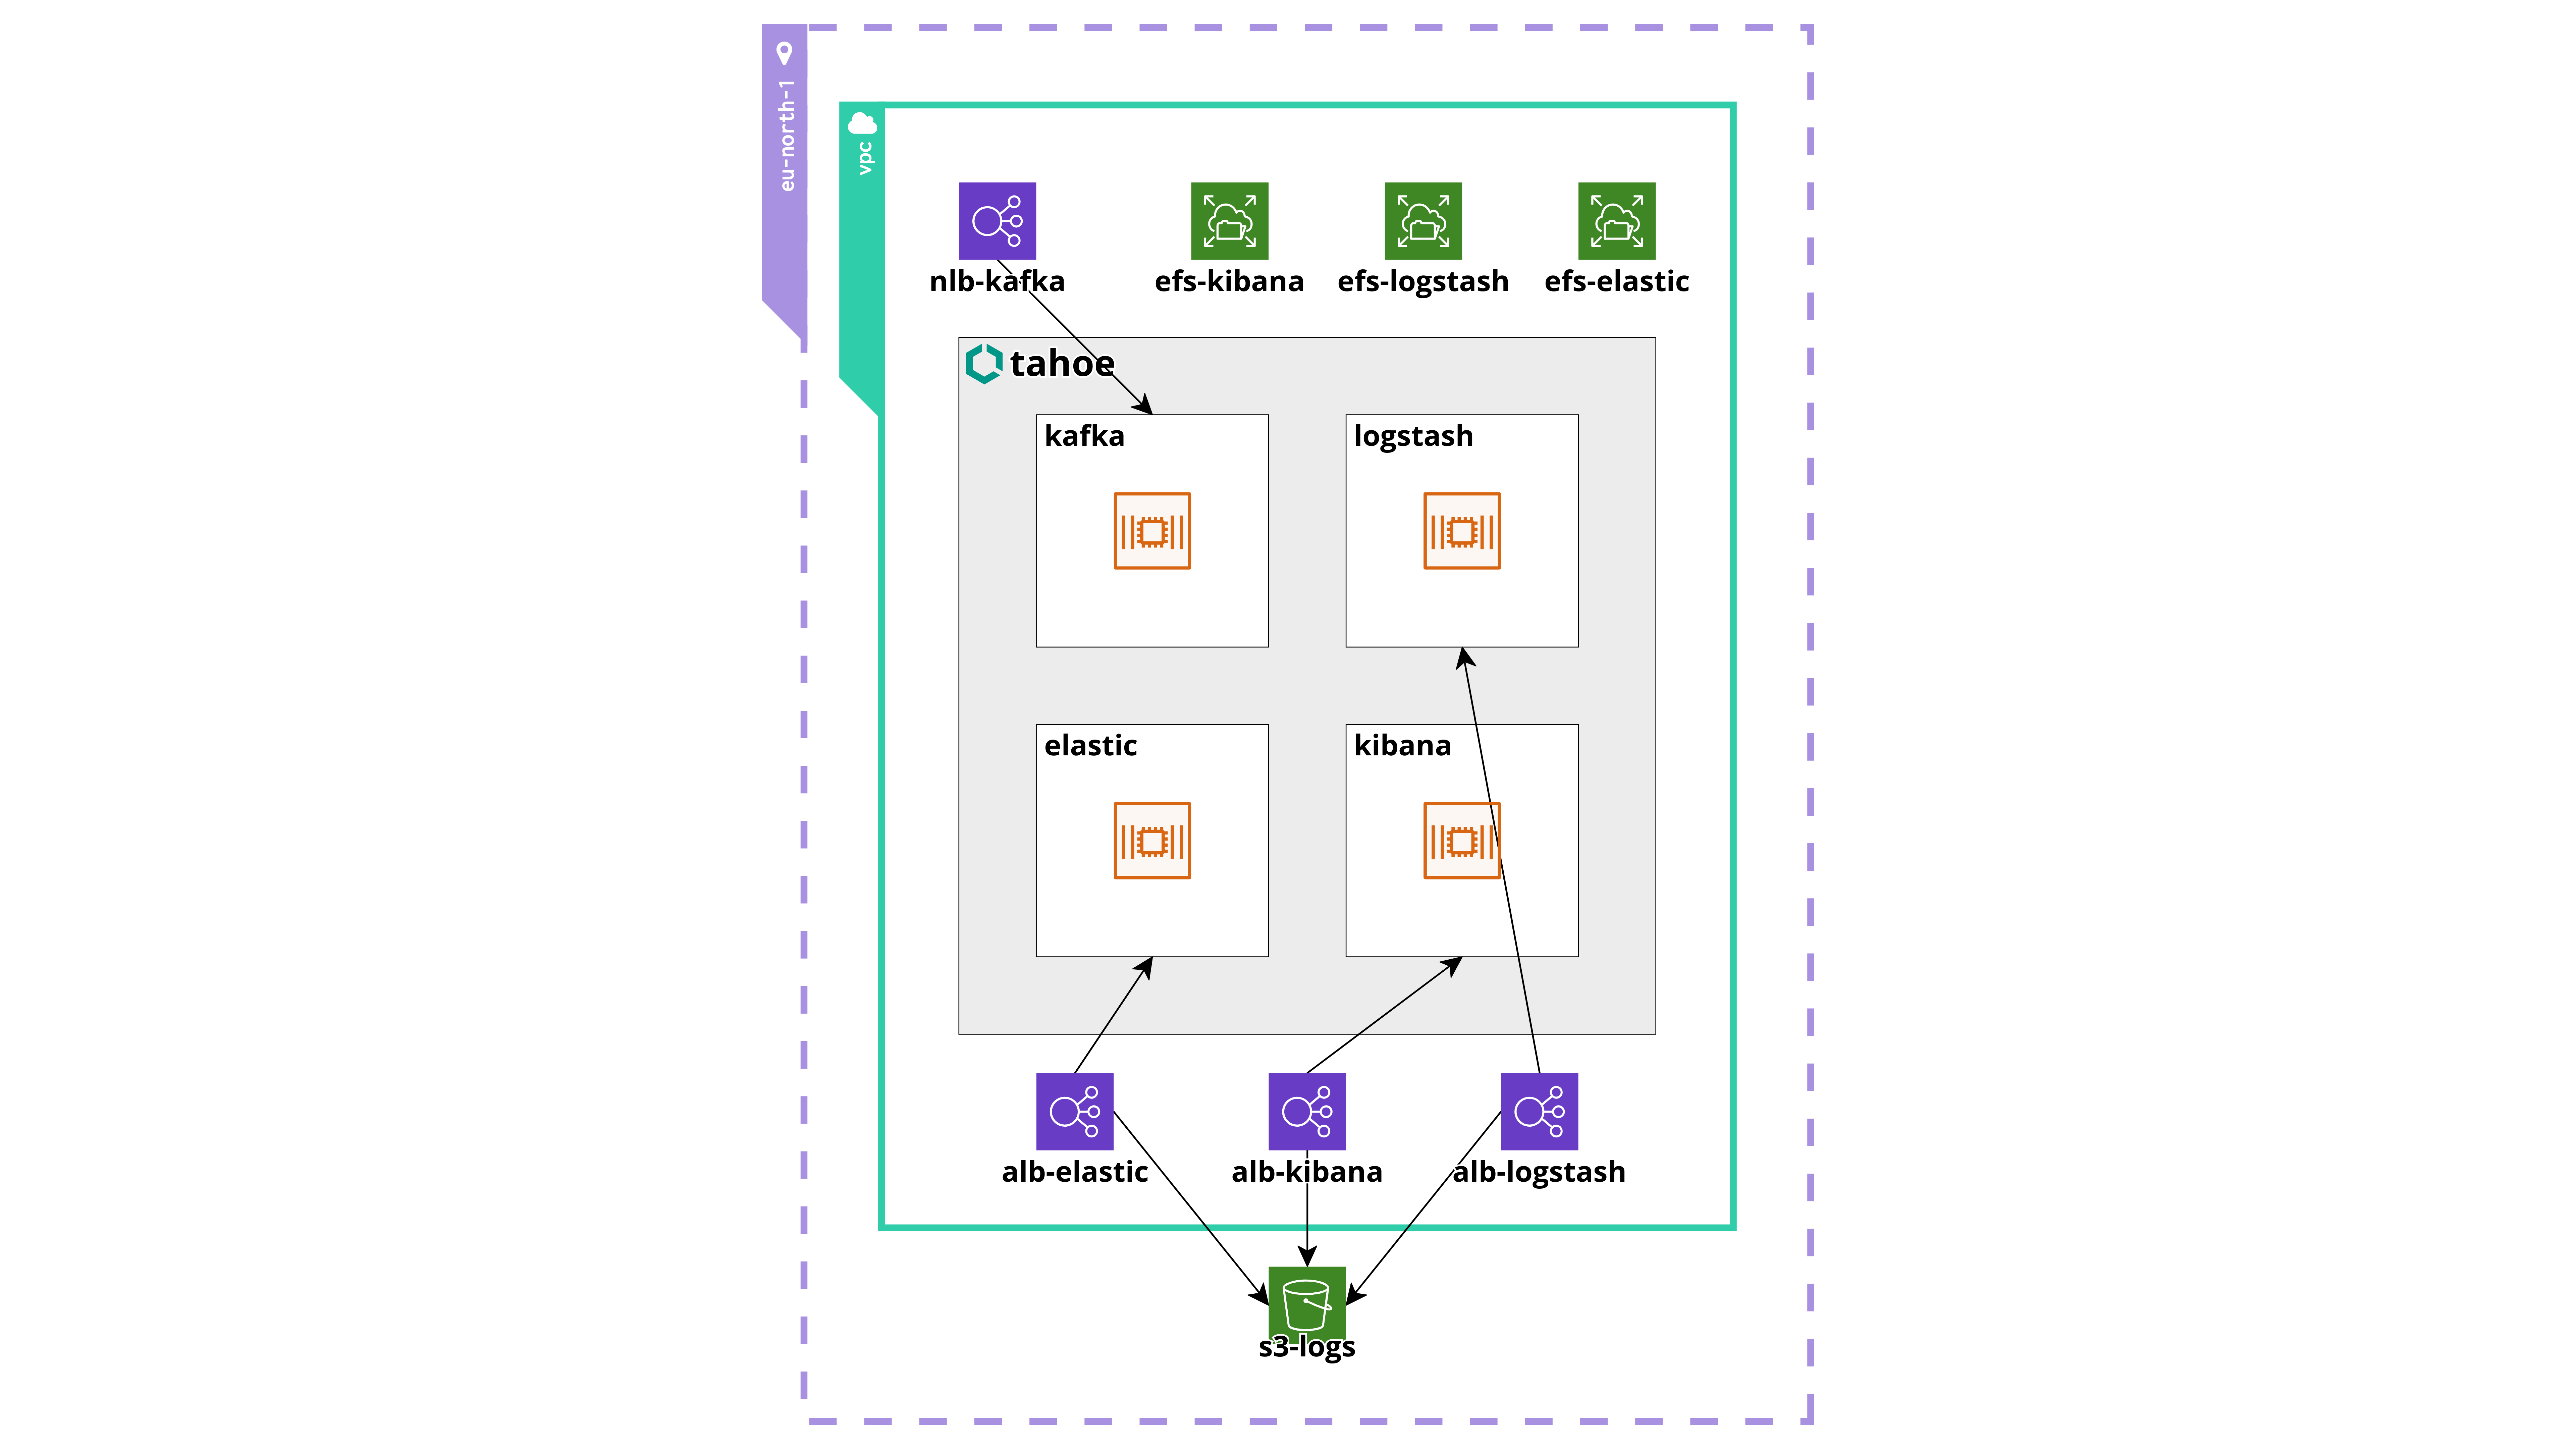
\includegraphics[width=1.3\textwidth]{aws_infra.png}}
	\caption{Diagrama inicial de la infraestructura en AWS}
	\label{fig:aws_infra}
\end{figure}

Los \textit{ALB} están conectados directamente a un ``caldero'' \textit{S3} que
almacena los logs de los servicios (\textit{NLB} no soporta esta funcionalidad).
Además, los servicios que necesiten almacenar datos de forma persistente (todos
menos Kafka) estarán conectados a un sistema de archivos \textit{EFS} que
permitirá compartir datos y configuraciones entre los contenedores del sistema.


\subsection{Seguridad}
A nivel de seguridad, se debe garantizar la protección de los datos y la
confidencialidad de la información. Para ello, se utilizarán varios servicios de
AWS, como \textit{IAM} para la gestión de roles y políticas de seguridad, o
\textit{grupos de seguridad} que permiten controlar el tráfico de red entre los
contenedores del sistema.

Cada uno de los componentes del \textit{clúster} de \textit{ECS} tendrá su
propio grupo de seguridad que permitirá controlar el tráfico de red según los
puertos y protocolos permitidos. Además, se deberán utilizar tan solo las
políticas y roles necesarios para garantizar la seguridad de los datos.

\begin{figure}[H]
	\centerline{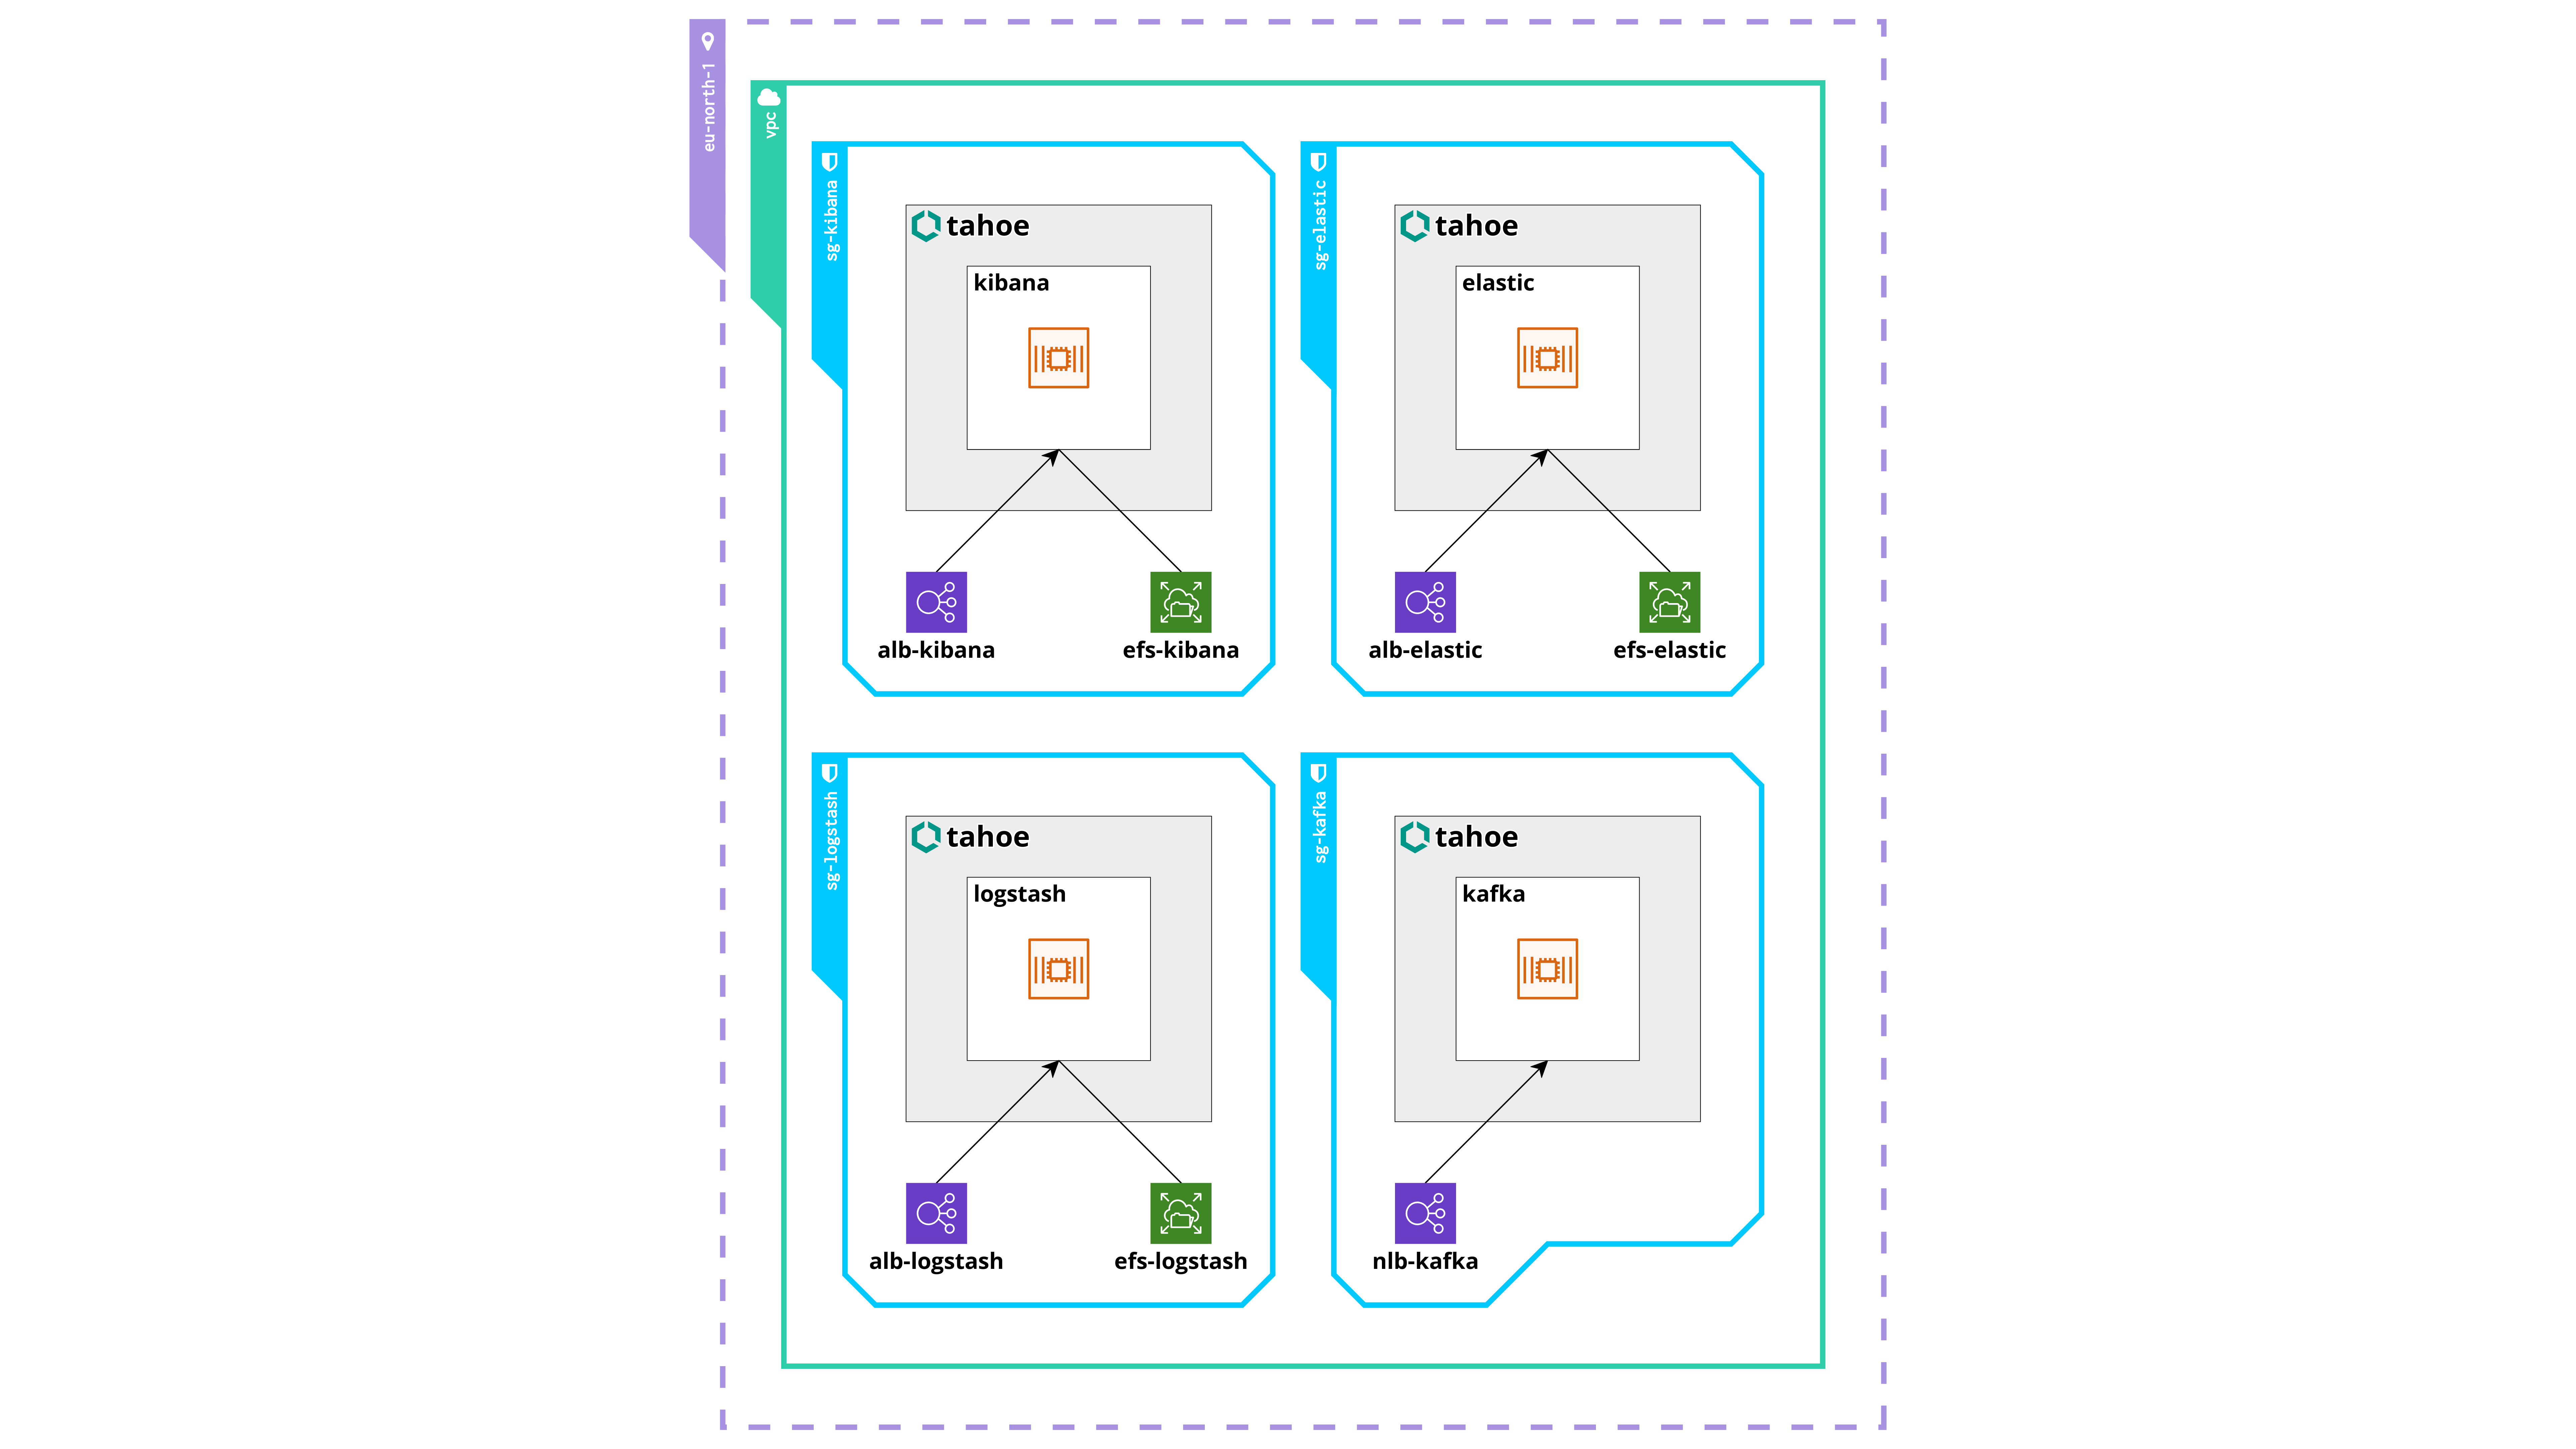
\includegraphics[width=1.3\textwidth]{aws_seguridad.png}}
	\caption{Diagrama incial de la seguridad en AWS}
	\label{fig:aws_seguridad}
\end{figure}

Además de los componentes de seguridad de AWS, se utilizarán protocolos seguros
como \textit{HTTPS} para la comunicación entre los servicios y se cifrará la
información sensible en reposo y en tránsito haciendo uso de
\textit{Secret Manager} para cargar y guardar las claves sensibles.


\subsection{Redes}
A nivel de configuración de redes, se establecen tres subredes: dos públicas y
otra privada, estando las públicas en zonas de disponibilidad diferentes. La
subred pública estará conectada a internet a través de un
\textit{Internet Gateway}, mientras que la subred privada estará conectada a
internet a través de un \textit{NAT Gateway}. Ambas subredes estarán conectadas
a una \textit{VPC} que permitirá la comunicación entre los servicios del
sistema.

\begin{figure}[H]
	\centerline{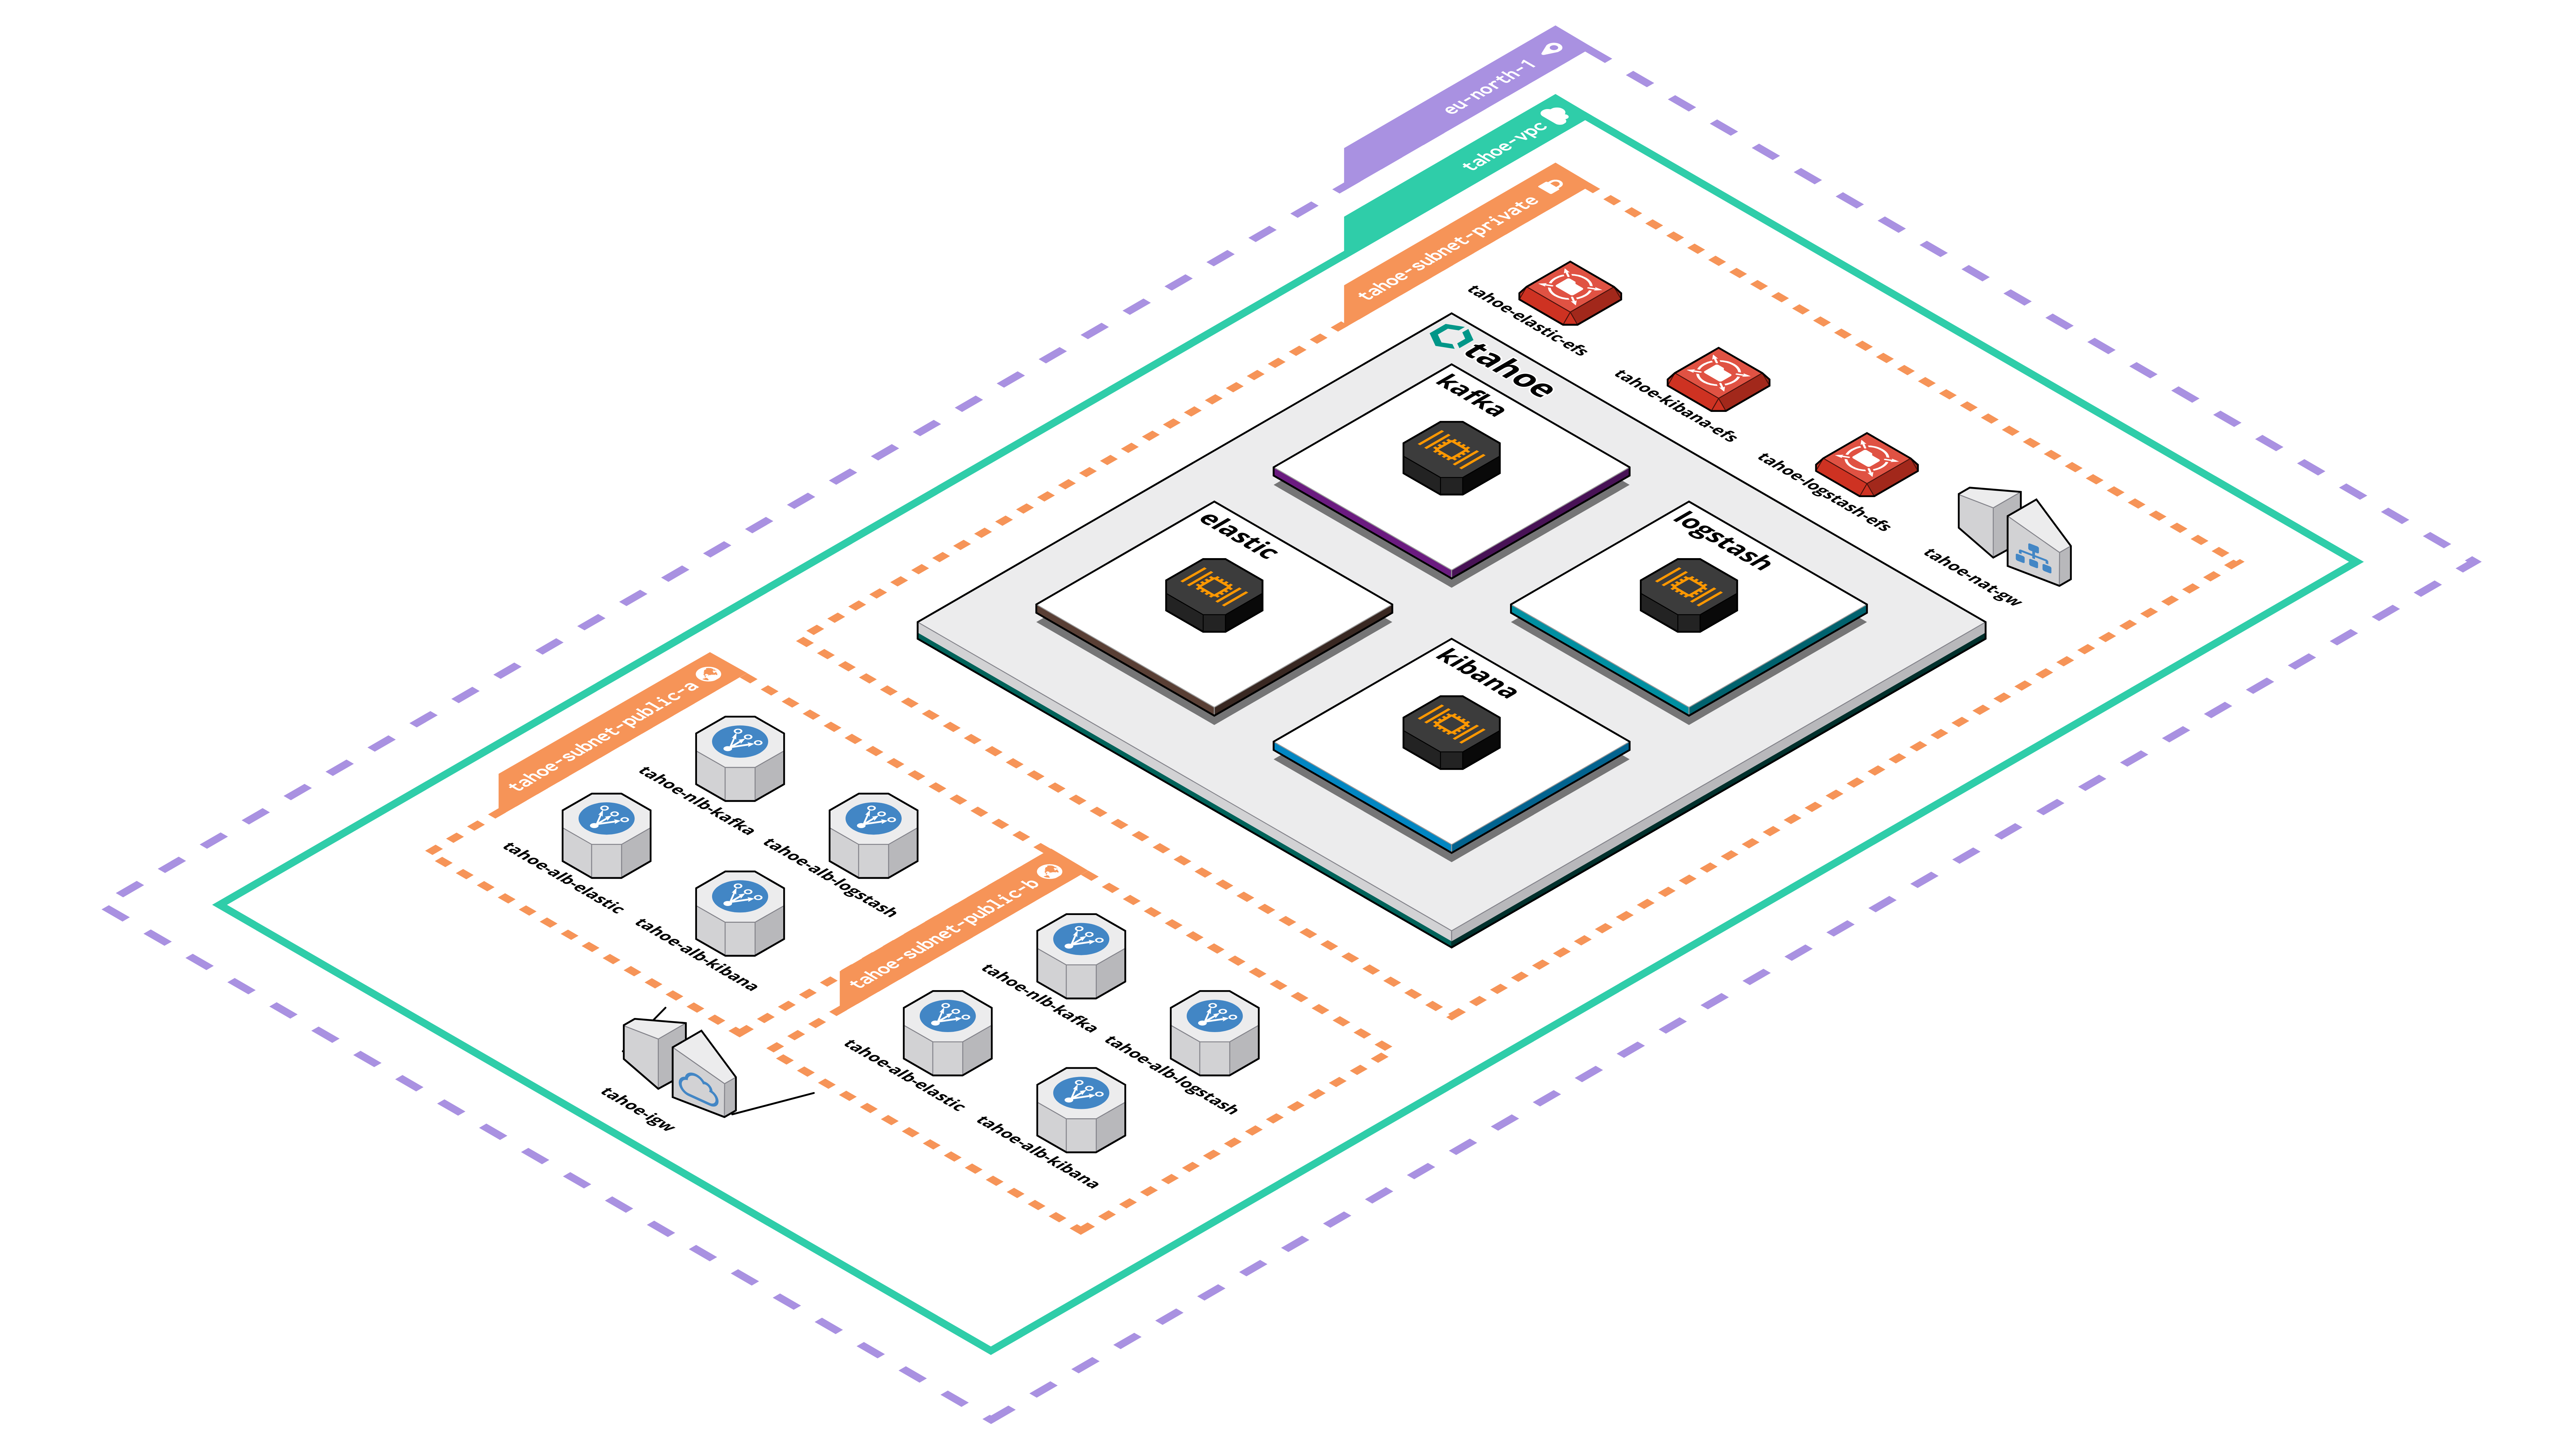
\includegraphics[width=1.3\textwidth]{aws_redes.png}}
	\caption{Diagrama incial de las redes en AWS}
	\label{fig:aws_redes}
\end{figure}

Además de los componentes planteados en el esquema anterior, se configurarán
\textit{rutas} y \textit{tablas de rutas} para garantizar la conectividad y la
seguridad de los servicios del sistema.


\newpage{}
\section{Modelos de datos}\label{sec:modelo}
